\section{SwitchCrypt Design} \label{sec:design}

\subsection{SwitchCrypt Overview} \label{subsec:overview}

\begin{figure}[ht]
   \centering
   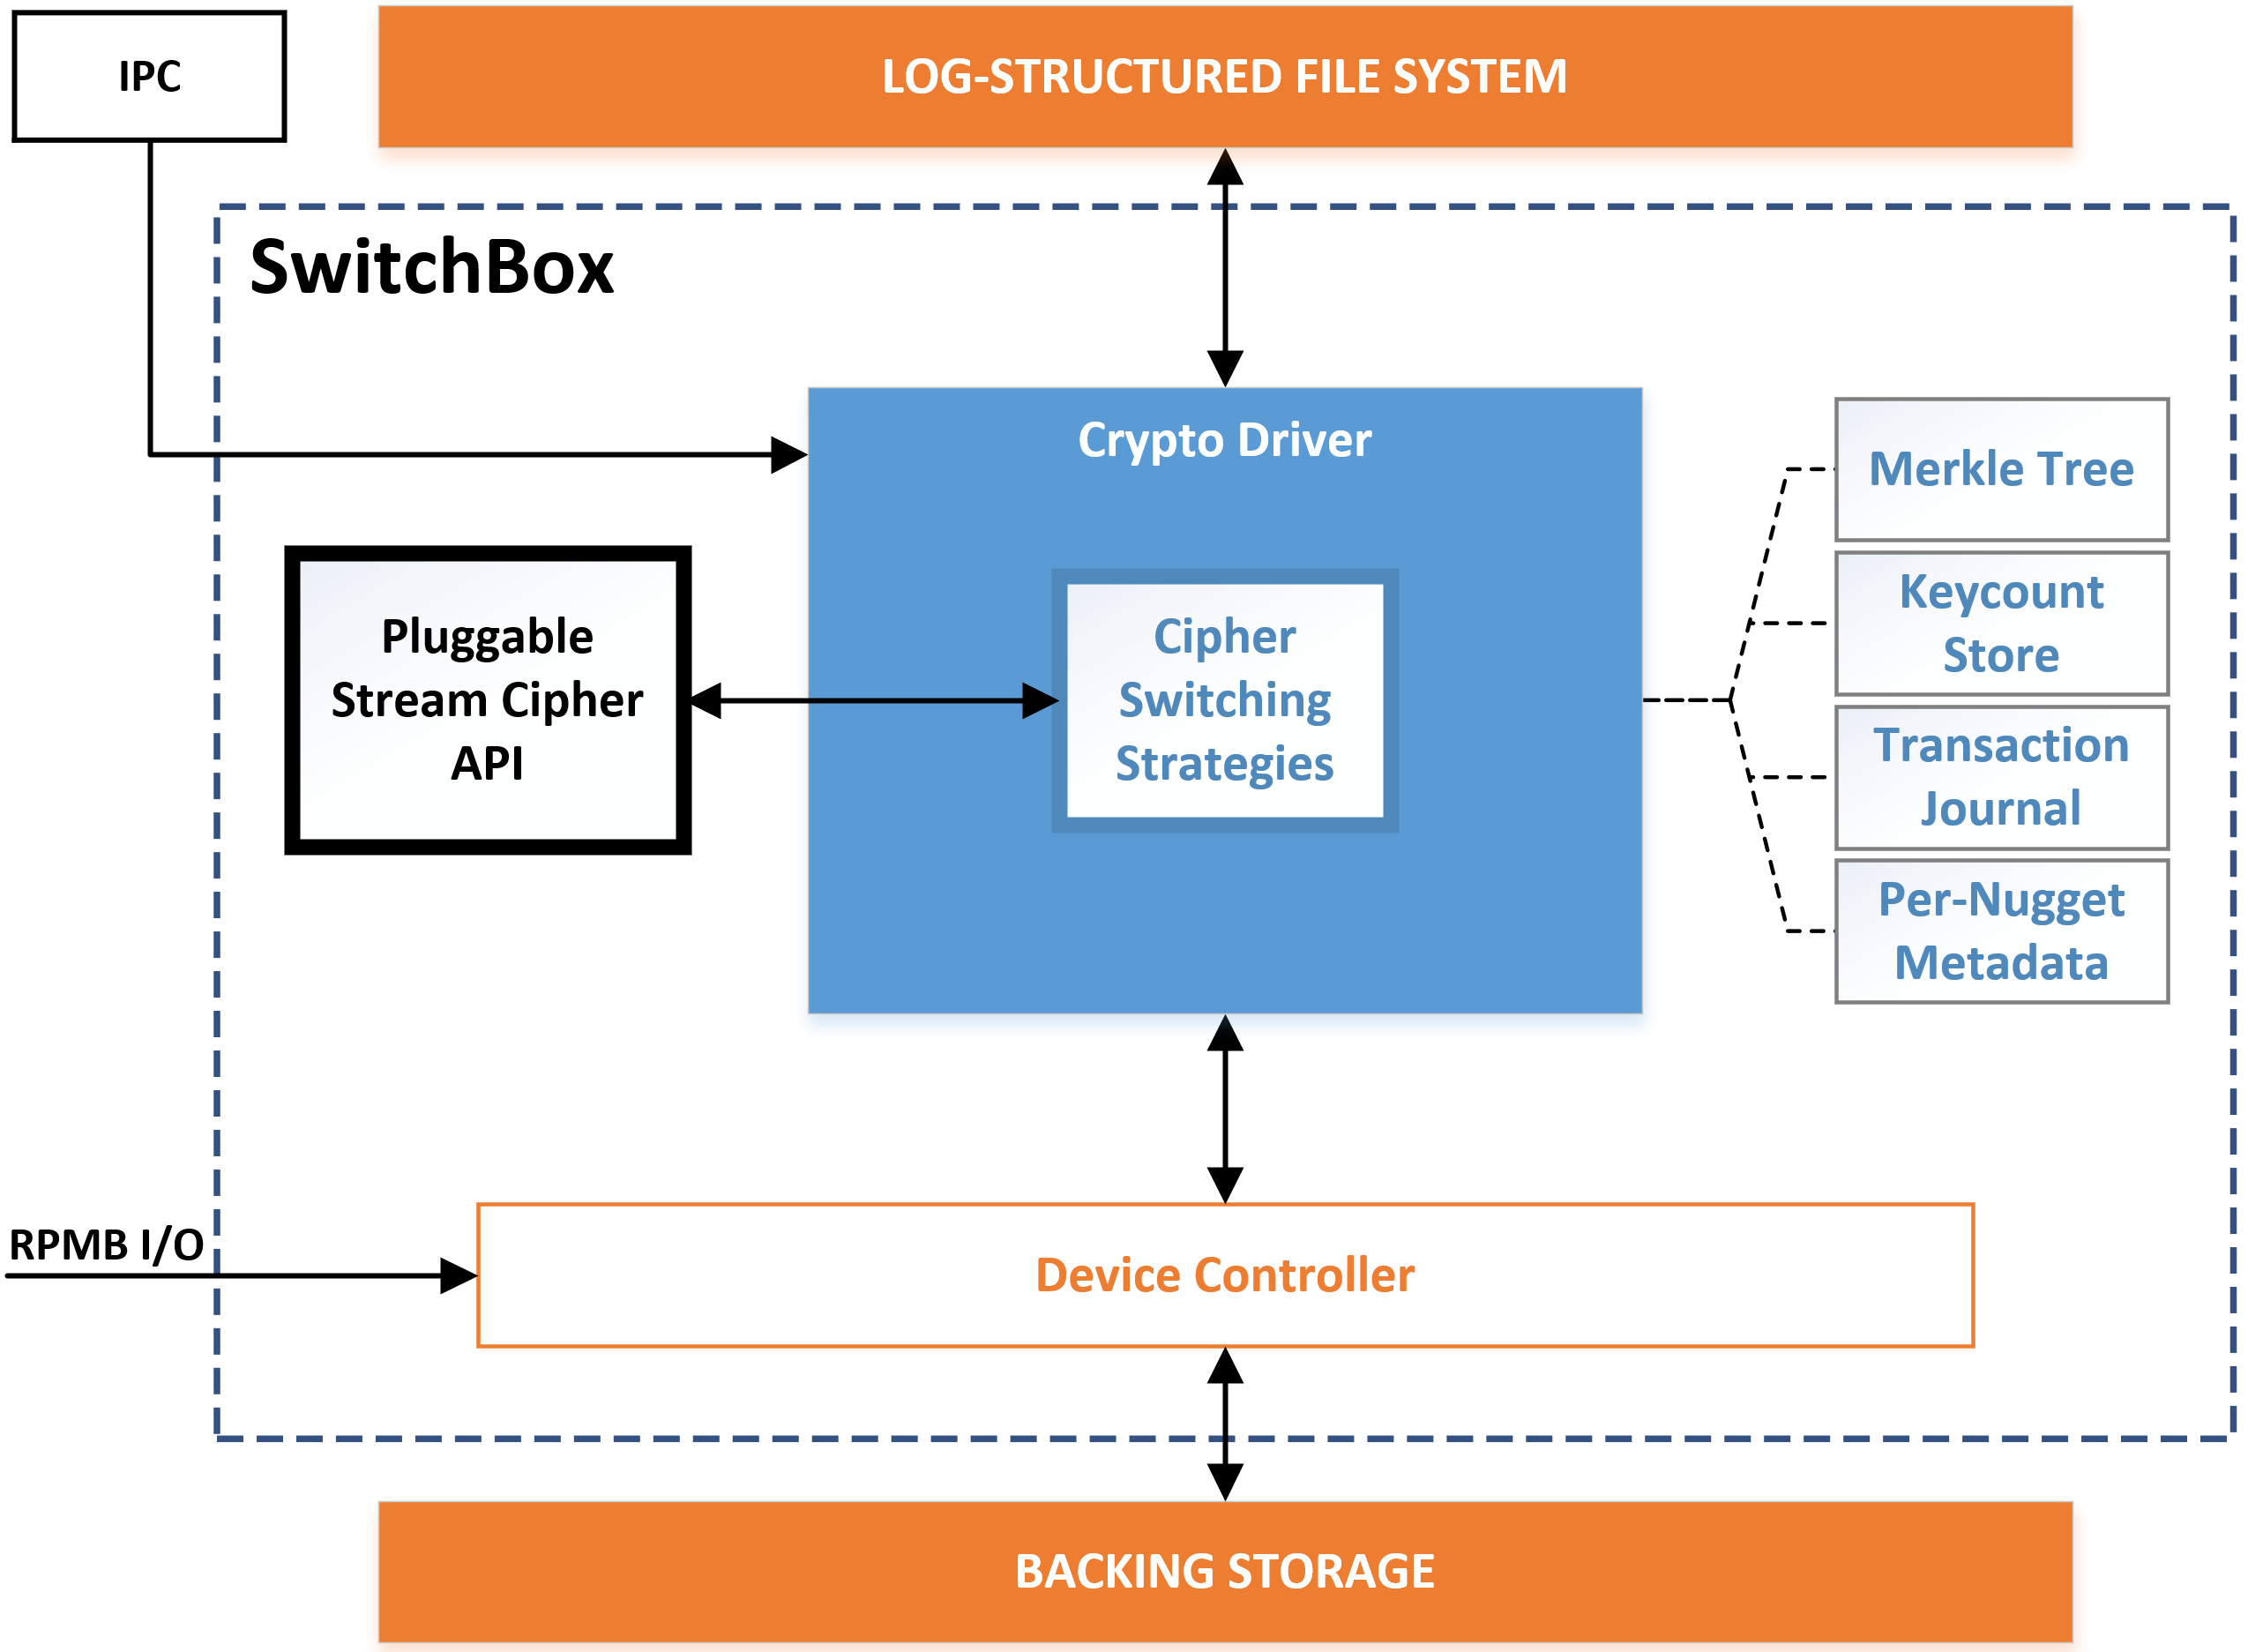
\includegraphics[width=\linewidth]{overview.png}
   \caption{Overview of the SwitchCrypt construction.} \label{fig:overview}
\end{figure}

SwitchCrypt consists of a \emph{Generic Stream Cipher Interface} and
\emph{Cryptographic Driver}; SwitchCrypt sits between a Log-structured File
System (LFS) on the OS, and the underlying drive (backing storage) and device
controller (e.g. Flash Translation Layer). This is illustrated in
\figref{overview}, which provides an overview of the SwitchCrypt system design.

\begin{figure}[t]
   \centering
   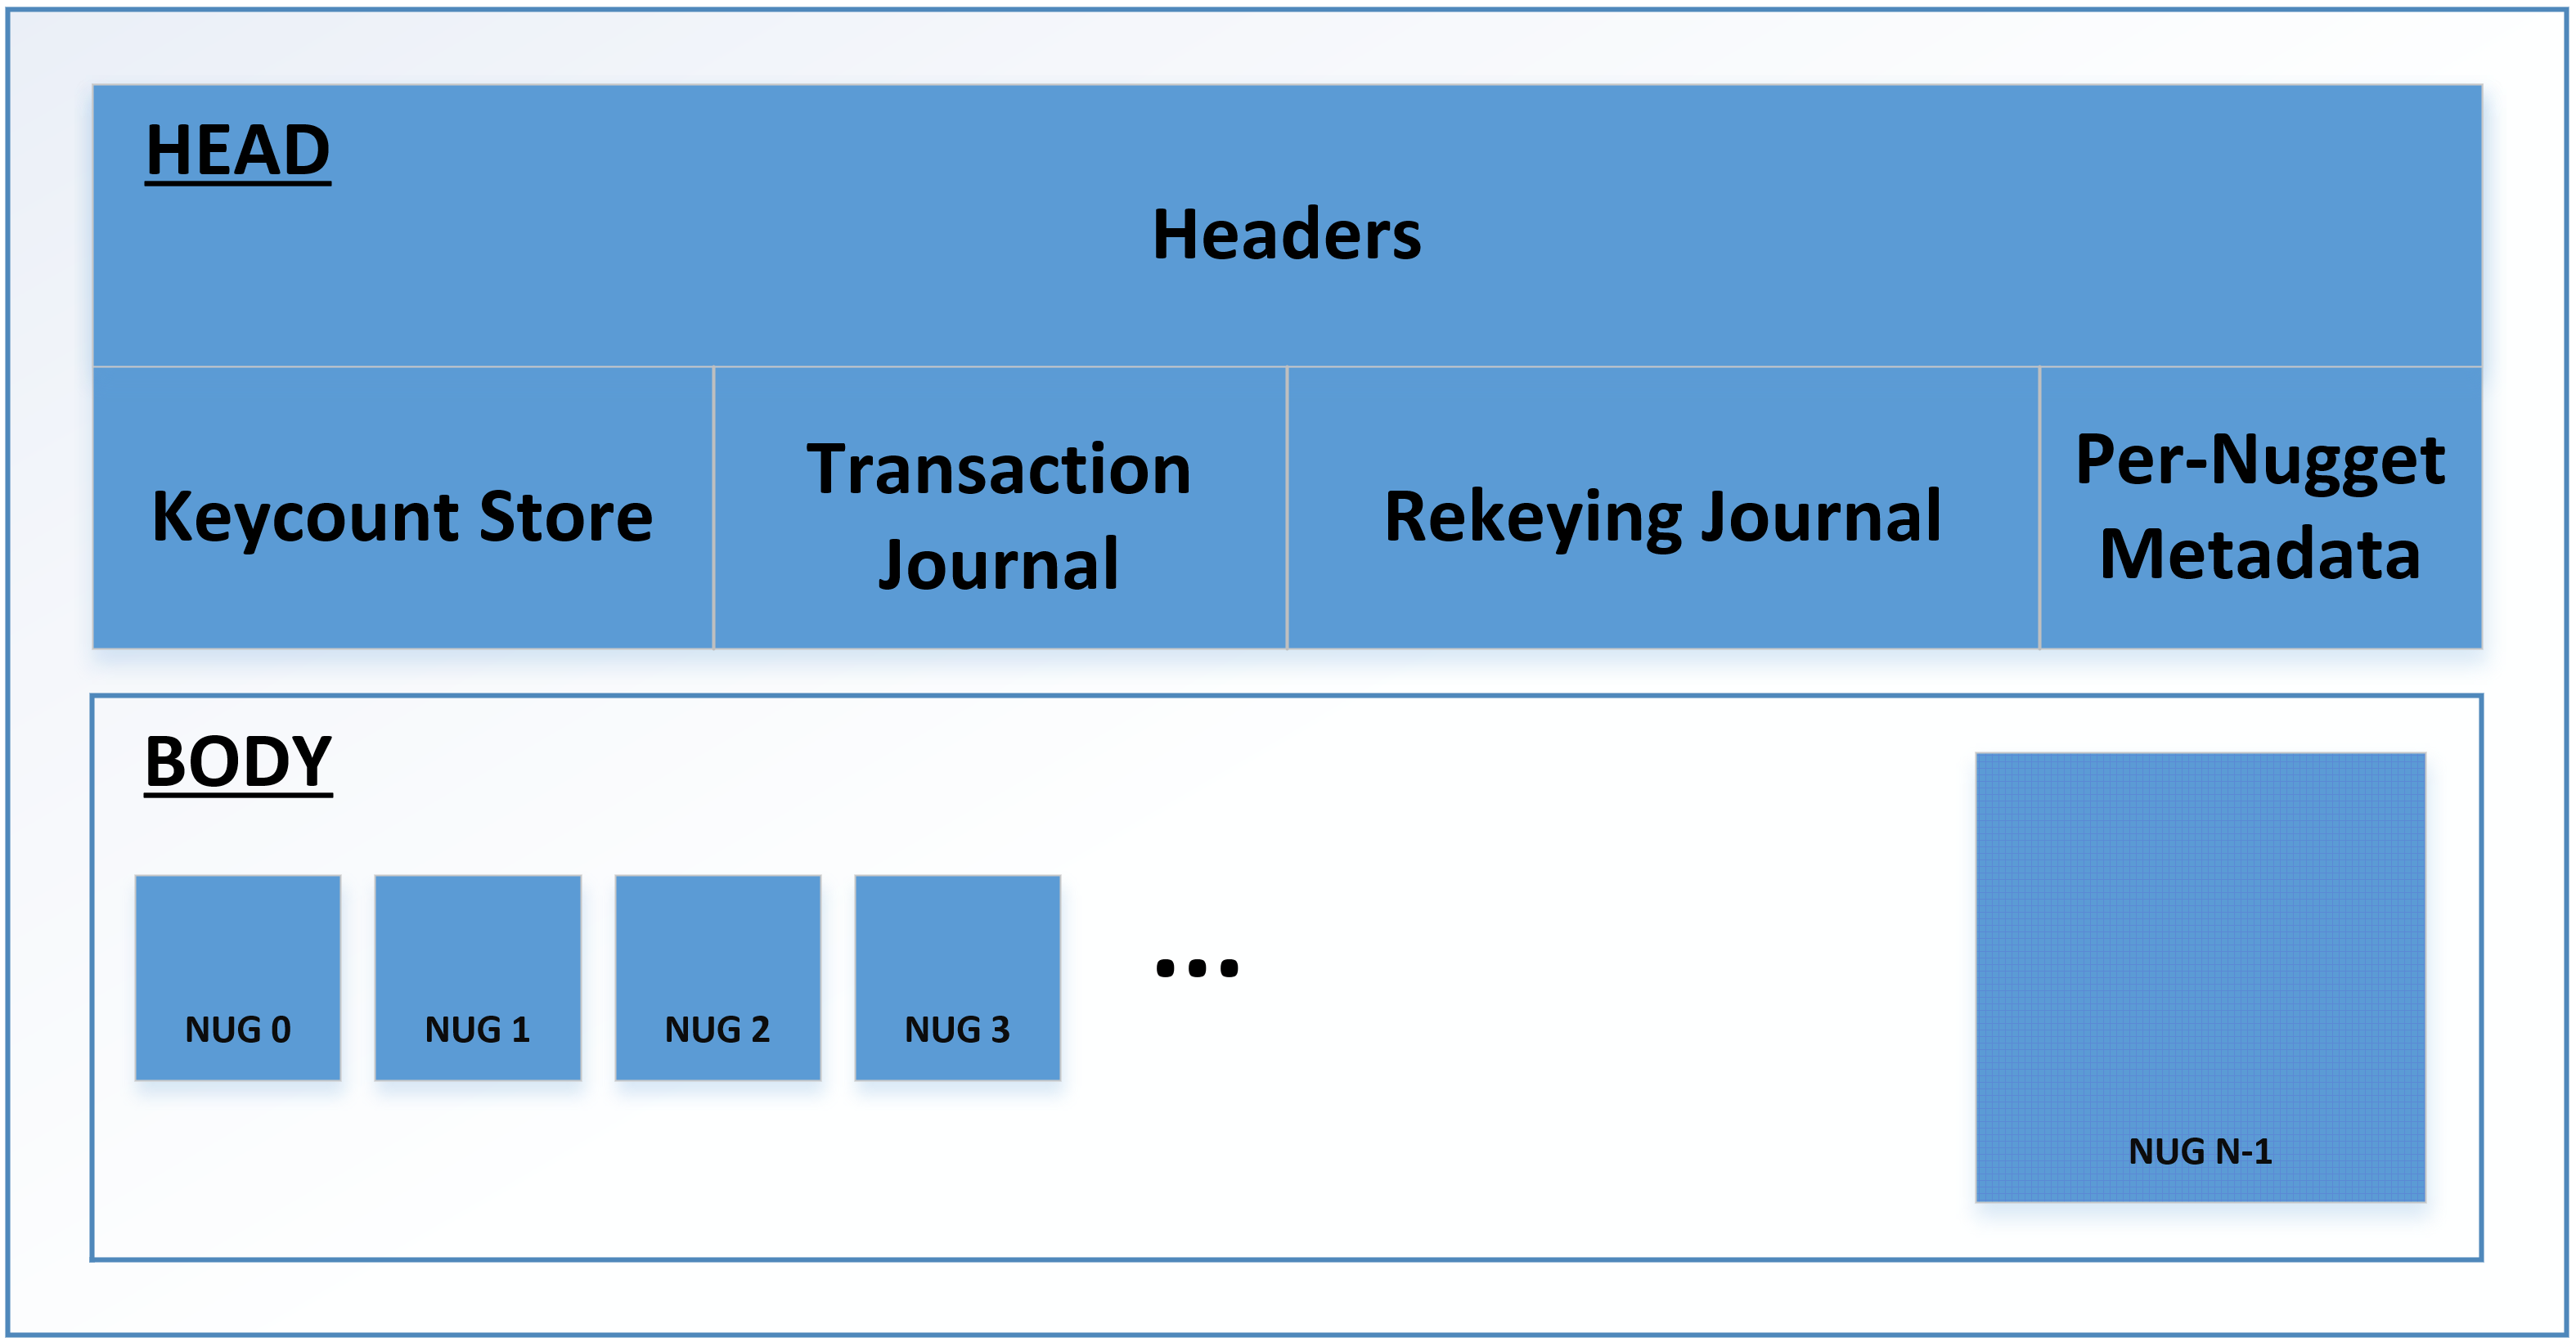
\includegraphics[width=\linewidth]{backstore.png}
   \caption{Layout of SwitchCrypt's drive layout.} \label{fig:backstore}
\end{figure}

The drive itself is divided into a \emph{HEAD} section and \emph{BODY} section
upon initialization, illustrated in \figref{backstore}. The HEAD consists of
metadata headers written during initialization~\cite{StrongBox} along with the
\emph{Keycount Store}, \emph{Transaction Journal}, \emph{Rekeying Journal}, and
\emph{Per-Nugget Metadata}, each drive-backed. These components are used by the
\emph{Cryptographic Driver} together with the \emph{Cipher Switching Strategy}
implementations to enable efficient per-unit cipher switching.

The BODY consists of a series independent same-size logical units called
\emph{nuggets}. A nugget consists of one or more contiguous physical drive
blocks. Each nugget is coupled with metadata in the HEAD indicating which cipher
was used to encrypt the nugget along with any additional ciphertext output; the
latter allows us to treat any non-length-preserving ciphers as if they were
length-preserving. SwitchCrypt uses the Keycount Store and Transaction Journal
components along with our nugget layout to 1) track, detect, and handle
overwrites, 2) limit the maximum length of any plaintext input to ciphers, thus
amortizing the overhead incurred during encryption, and 3) independently and
efficiently switch the cipher used to encrypt individual nuggets.

Dickens et al. showed how to make nugget-based drive organization secure using a
single stream cipher, ChaCha20, to handle overwrites, prevent rollback attacks,
and limit plaintext length~\cite{StrongBox}. However, they did not envision the
utility in trading off between concerns at the filesystem or device-mapper
level, dynamic cipher switching, or protecting against attacks on data ``in
motion;'' the remainder of this section details the novel components that enable
this functionality. Specifically: how we quantify the properties traded off
between configurations (\cref{subsec:quantify}), the Generic Stream Cipher
Interface and Per-Nugget Metadata components (\cref{subsec:interface}) which
decouple cipher implementations from the encryption process, and our Cipher
Switching Strategy implementations (\cref{subsec:strategies}) used to
efficiently encrypt nuggets with different ciphers.

\subsection{Quantifying Cipher Security Properties} \label{subsec:quantify}

To reason about when to trade off between the ciphers evaluated in this work, we
must have a way to compare ciphers' utility in the context of SwitchCrypt FDE.
However, different ciphers have a wide range of security properties, performance
profiles, and output characteristics. To address this need, we propose a novel
evaluation framework (see: \tblref{security-quant}). Our framework classifies
stream ciphers according to three quantitative features: relative round count,
ciphertext randomization, and ciphertext expansion. Taken together, these
features reveal a rich tradeoff space of cipher configurations optimizing for
different combinations of concerns.

\begin{table}[ht]
   \begin{tabular}{@{}ccccc@{}}
   \toprule
   \textbf{Cipher} & \textbf{Rounds} & \textbf{Randomization} &
   \textbf{Expansion} \\
   \midrule
   ChaCha8         & 0           & 0           & 1           \\
   ChaCha12        & 0.5         & 0           & 1           \\
   ChaCha20        & 1           & 0           & 1           \\
   Salsa8          & 0           & 0           & 1           \\
   Salsa12         & 0.5         & 0           & 1           \\
   Salsa20         & 1           & 0           & 1           \\
   HC128           & 0           & 0           & 1           \\
   HC256           & 1           & 0           & 1           \\
   Freestyle (F)   & 0           & 2           & 0           \\
   Freestyle (B)   & 0.5         & 2.5         & 0           \\
   Freestyle (S)   & 1           & 3           & 0           \\
\end{tabular}
   \caption{Our framework for classifying stream ciphers according to three
   ideal features: relative round count, ciphertext randomization, and
   ciphertext expansion.}
   \label{tbl:security-quant}
 \end{table}

\subsubsection{Relative Rounds (Rounds)}

The ciphers we examine in this paper are all constructed around the notion of
\emph{rounds}, where a higher number of rounds (and possibly longer key) is
positively correlated with a higher resistance to brute force given no fatal
related-key or other attacks~\cite{ChaCha-Cryptanalysis}. Hence, this feature
represents how many rounds a cipher executes relative to other implementations
of the same algorithm. For instance: ChaCha8 is a reduced-round version of
ChaCha12, which is a reduced-round version of ChaCha20, all using the ChaCha
algorithm~\cite{ChaCha20,ChaCha-Cryptanalysis}.

We limit our analysis to groups of three implementations, each using a different
number of rounds. In the case of HC-128 and HC-256, we limit our analysis to a
group of two implementations. Scores range from 0 (least number of rounds
considered) to 1 (greatest number of rounds considered).

\subsubsection{Ciphertext Randomization (Randomization)}

A cipher with ciphertext randomization generates different ciphertexts
non-deterministically given the same key, nonce, and plaintext. This makes it
much more difficult to execute chosen-ciphertext attacks (CCA), key
re-installation attacks, XOR-based cryptanalysis and other comparison attacks,
and other confidentiality-violating schemes where the ciphertext is in full
control of the adversary ~\cite{Freestyle}. This property is useful in cases
where we cannot prevent the same key, nonce, and plaintext from being reused,
such as with data ``in motion'' (see the motivational example earlier in this
work). Ciphers without this property---such as ChaCha20 on which prior work is
based---are trivially broken when key-nonce-plaintext 3-tuples are reused. In
StrongBox, this is referred to as an ``overwrite condition'' or simply
``overwrite''~\cite{StrongBox}.

Though there are many ways to achieve ciphertext randomization, the ciphers
included in our analysis implement it using a random number of rounds for each
block of the message where the exact number of rounds are unknown to the
receiver a priori~\cite{Freestyle}. In determining the minimum and maximum
number of rounds used per block in this non-deterministic mode of operation, we
can customize the computational burden an attacker must bear by choosing lower
or higher minimums and maximums. Hence, this is not a binary feature; scores
range from 0 (no ciphertext randomization) to 1 (lowest minimum and maximum
rounds per block) to 3 (highest minimum and maximum rounds per block).

\subsubsection{Ciphertext Expansion (Expansion)}

A cipher that exhibits ciphertext expansion is non-length-preserving: it outputs
more or less ciphertext than was originally input as plaintext. This can cause
major problems in the FDE context. For instance, cryptosystems that rely on
AES-XTS (e.g. Linux's dm-crypt, Microsoft's BitLocker, Apple's FileVault) or
ChaCha (e.g. StrongBox, Google's Adiantum) have storage layouts that hold
length-preserving output as an invariant, making ciphers that do not exhibit
this property incompatible with their implementations; yet, ciphertext expansion
is often (but not always) a necessary side-effect of ciphertext randomization.

The ciphers included in our analysis that exhibit ciphertext expansion have an
overhead of around 1.56\% per plaintext message block~\cite{Freestyle}. Even a
single byte of additional ciphertext vs plaintext would make a cipher
inappropriate for use with prior work. Hence, this is a binary feature in that a
cipher either outputs ciphertext of the same length as its plaintext input or it
does not. A cipher scores either a 0 if it \emph{is not} length-preserving in
this way or a 1 if the ciphertext is always the same length as the plaintext.

\subsection{Generic Stream Cipher Interface} \label{subsec:interface}

One of the goals of SwitchCrypt is that we might use any stream cipher
regardless of its implementation details. Yet this is entirely non-trivial.
There are many cipher implementations that we might use with SwitchCrypt, each
with unique input requirements and output considerations. For instance, Salsa
and Chacha implementations require a certain IV and key size and handle
plaintext input through successive invocations of a single state update
function~\cite{Floodyberry}. Using OpenSSL's AES implementation in CTR mode
requires manually tracking the counter state and individual ciphertext blocks
are retrieved though corresponding function invocations~\cite{OpenSSL}.
Freestyle's reference implementation requires we calculate the extra space
necessary per nugget (due to ciphertext expansion) along with
configuration-dependent minimum and maximum rounds-per-block, hash interval, and
pepper bits~\cite{Freestyle}. HC-128 and other ciphers have similarly disparate
requirements.

Unlike prior work, SwitchCrypt must be able to encrypt and decrypt arbitrary
nuggets \emph{with any of these ciphers} at any moment with low overhead and
without tight coupling to any specific implementation detail. Hence, there is a
need for an interface that completely decouples cipher implementations from the
encryption/decryption process. Our novel cipher interface allows any stream
cipher to be integrated into SwitchCrypt without modifications to third-party
code, enabling normally incompatible ciphers to encrypt and decrypt arbitrary
nuggets. The ability for disparate cipher implementations to co-exist forms the
foundation for SwitchCrypt's ability to switch the system between different
cipher configurations in our tradeoff space efficiently and effectively.

To facilitate this, the Generic Stream Cipher Interface presents the
cryptographic driver with a single unified encryption/decryption model.
SwitchCrypt receives I/O requests from the operating system at the block device
level like any other device-mapper. These requests come in the form of either
reads or writes. When a read request is received, the OS hands SwitchCrypt an
offset and a length and expects a response with plaintext of that specific
length starting at that specific offset taken from the beginning of storage
(i.e. the BODY section; see \figref{backstore}). When a write request is
received, the OS hands SwitchCrypt an offset, a length, and a buffer of
plaintext and expects that plaintext to be encrypted and committed to storage
such that the plaintext is later retrievable given that same offset and length
in a future read request. These requests can either be handled together by a
single function or handled individually as distinct read and write operations,
each with different tradeoffs.

\begin{enumerate}
   \item \textbf{\texttt{xor\_interface}}\\\texttt{xor\_interface} executes
   independently of SwitchCrypt internals and treats encryption and decryption
   as the same operation. Implementations receive an integer offset $F$, an
   integer length $L$, a key buffer $K$ corresponding to the current nugget, and
   an empty $L$-length XOR buffer. SwitchCrypt expects the XOR buffer to be
   populated with $L$ bytes of keystream output from some stream cipher seeked
   to offset $F$ with respect to key $K$. The length of the key buffer will
   always be exactly what the cipher implementation expects, alleviating the
   burden of key management; similarly, the XOR buffer will be XOR-ed with the
   appropriate portion of nugget contents automatically, alleviating the burden
   of drive access and other tedious calculations. \\
   \item \textbf{\texttt{read\_interface}} and
   \textbf{\texttt{write\_interface}}\\
   Unlike \texttt{xor\_interface}, encryption and decryption are distinct
   concerns at this abstraction level. \\\texttt{read\_interface} handles
   decryption during reads. \\\texttt{write\_interface} handles encryption
   during writes. Implementations receive full access to SwitchCrypt internals,
   giving wrapper code complete control over the encryption and decryption
   process and allowing implementers to bypass parts of the nugget-based drive
   layout abstraction (i.e. BODY) if necessary. This comes at the cost of 1)
   significantly increased code complexity, as the implementer must perform
   certain I/O manually, distinguish between independent nuggets on the drive,
   determine what to encrypt or decrypt at what offset and when, when to commit
   which metadata and where and 2) potential performance implications, since
   SwitchCrypt must account for not having absolute control over its internal
   data structures during function invocation. For a cipher like Freestyle,
   configurations with lower minimum and maximum rounds per block may see a
   performance improvement here, while configurations with higher minimum and
   maximum rounds per block may see reduced performance.
\end{enumerate}

\subsection{Cipher Switching Strategies} \label{subsec:strategies}

The Generic Stream Cipher Interface allows many differently ciphered nuggets to
co-exist on the same drive. However, at any moment, there is only a single
\emph{active cipher configuration} (henceforth \emph{active configuration}). The
active configuration is used to encrypt nugget contents. When a cipher switch is
triggered, a different configuration becomes the active configuration. At this
point, SwitchCrypt must determine \emph{when} to re-cipher a nugget and
\emph{where} to store the output on the drive. ``Re-ciphering'' here means using
an inactive configuration to decrypt a nugget's contents and using the active
configuration to re-cipher it. Depending on the use case, it may make the most
sense to re-cipher a nugget immediately, or eventually, or to maintain several
areas of differently-ciphered nuggets concurrently.

A naive approach would switch every nugget in BODY to the active configuration
immediately, but the latency and energy cost would be unacceptable. Hence, a
more strategic approach is necessary. We satisfy this need with our \emph{cipher
switching strategies}. These novel strategies allow for nuggets to be
re-ciphered in a variety of cases with minimal impact on performance and battery
life and without compromising security. This is thanks to the nugget-based drive
layout, which limits the churn of cipher switching operations to relatively
small regions of ciphertext on the drive.

Determining \emph{when} to target a nugget for re-ciphering we call
\emph{temporal switching}, for which we propose the \emph{Forward} switching
strategy. Determining \emph{where}---in which storage region and across which
nuggets---to output ciphertext we call \emph{spatial switching}, for which we
propose the \emph{Mirrored} and \emph{Selective} switching strategies.

\textbf{Forward Switching Strategy.} When a nugget is encountered during I/O
that was encrypted using something other than the active configuration, the
Forward strategy dictates that this nugget be re-ciphered immediately. If a
particular nugget encrypted with an inactive configuration is never encountered
during I/O, it is never re-ciphered and remains on the drive in its original
state. In this way, the Forward strategy represents a form of temporal cipher
switching.

Rather than re-cipher the entire drive every time the active configuration
changes, this strategy limits the performance impact of cipher switching to
individual nuggets. The expense of re-ciphering is paid only once, after which
the nugget is accessed normally during I/O until the active configuration is
switched again.

\PUNT{There are several forms the Forward strategy might take. The default and
most intuitive is \emph{0-forward}, in which SwitchCrypt immediately transitions
individual nuggets encountered during I/O to the active configuration if they
are not using it. Over time, if various I/O operations end up touching every
nugget in the drive, the encrypted contents of every nugget will become
decryptable with the currently active configuration.

The Forward strategy might also take the form of \emph{N-forward}, where
SwitchCrypt attempts to take advantage of spatial sequential locality to
transition whole sets of nuggets into the active configuration. We can trivially
expand the forward strategy to encompass the entire drive by selecting $N$ equal
to the total number of nuggets managed by SwitchCrypt. This would have the
overhead of re-ciphering large swaths of the drive upon every I/O operation
where a nugget encrypted with the inactive configuration is encountered. Of
course, this has the same dire implications for performance as simply
re-initializing the entire system or encrypted container with the new cipher.}

\textbf{Selective Switching Strategy.} When SwitchCrypt is initialized with the
Selective strategy, the drive is partitioned into $C$ regions where $C$
represents the total number of available ciphers in the system; each regions'
nuggets are encrypted by each of the $C$ ciphers respectively. For instance,
were SwitchCrypt initialized using two ciphers ($C = 2$), the drive would be
partitioned in half; all nuggets in the first region would be encrypted with the
first cipher while all nuggets in the second would be encrypted with the other.


When using this strategy, the active cipher determines which partition we
``select'' for I/O operations. Hence, unlike the Forward strategy, which
schedules individual nuggets to be re-ciphered at some point in time after the
active configuration is switched, the Selective strategy allows the wider system
to indicate \emph{where} on the drive a read or write operation should occur. In
this way, the Selective strategy represents a form of spatial cipher switching
where different regions of the drive can store differently-ciphered nuggets
independently and concurrently. A user could take advantage of this to, for
instance, set up regions with different security properties and performance
characteristics, managing them as distinct virtual drives or transparently
reading/writing bytes to different security regions on the same drive.

\textbf{Mirrored Switching Strategy.} Similar to the Selective strategy, when
SwitchCrypt is initialized with the Mirrored strategy, the drive is partitioned
into $C$ regions where $C$ represents the total number of available ciphers in
the system; each regions' nuggets are encrypted by each of the $C$ ciphers
respectively.

However, unlike the Selective strategy, all write operations that hit one region
are mirrored into the other regions immediately, so all regions of the drive
will always be in a consistent state and always share the same data. The active
configuration determines \emph{where} a read operation should occur. In this
way, the Mirrored strategy represents a form of spatial cipher switching because
we are switching which configuration we are using to read in data. A user could
take advantage of this along with SSD Instant Secure Erase~\cite{ISE1,ISE2,ISE3}
to delete other regions, thus quickly and securely converging the drive to a
single configuration without losing any data or suffering the egregious
performance or battery penalty that comes with re-ciphering every nugget.

\subsubsection{Comparing Cipher Switching Strategies}

\begin{table}[ht]
   \begin{tabular}{@{}|c|c|c|C{25mm}|@{}}
      \toprule
      \textbf{Strategy} & \textbf{Convergence} & \textbf{Waste} &
      \textbf{Performance} \\
      \midrule
      Forward   & Slower       & None & Faster reads and writes unless switching
      \\\hline
      Mirrored  & Nearly instant & High & Faster reads; slower writes \\
      \hline
      Selective & Slower       & High & Faster reads and writes  \\
      \hline
   \end{tabular}
   \caption{A summary comparison between the three cipher switching strategies.}
   \label{tbl:strategies-advantages}
\end{table}

\tblref{strategies-advantages} summarizes the higher level tradeoffs between the
three cipher switching strategies.

\textbf{Convergence.} Depending on the use case, the ability to quickly converge
the entire drive to a single cipher configuration without losing data is very
useful (see: \secref{usecases}). The near-instantaneous ``just forget the key''
nature of SSD Instant Secure Erase (ISE) implementations on modern
SSDs~\cite{ISE1,ISE2,ISE3} makes this a very fast process for the Mirrored
strategy. The Forward strategy is slow to converge compared to Mirrored since,
in the worse case, every nugget on the drive will require re-ciphering. The
Selective strategy is similarly slow to converge since entire regions of nuggets
must be moved and re-ciphered to prevent data loss; those regions could be
destroyed without moving data around using ISE too, which would be very fast,
but unlike Mirrored some data would be lost forever.

\textbf{Waste.} Unlike the other two strategies, using the Forward strategy does
not reduce the total usable space on the drive by the end-user, ciphertext
expansion notwithstanding. We refer to this as ``waste''. The Forward strategy
is not wasteful in this way because it allows differently-ciphered nuggets to
co-exist contiguously on the drive without special partitions. Since the
Mirrored and Selective strategies require partitioning the drive into some
number of regions---where the writeable size reported back to the OS is some
function of region size---there is a necessary reduction in usable space.

\textbf{Performance.} The Selective and Mirrored strategies can read data from
the drive with low overhead, reaching performance parity with prior work,
because they never have to deal with on-demand re-ciphering. This is because
switching ciphers using these two strategies amounts to offsetting the read
index so that it lands in the proper BODY partition on the drive, which has
little overhead. The Forward strategy also reads with low overhead except in the
case where a nugget was not encrypted with the active configuration. This
triggers re-ciphering on-demand, which can be costly if the workload constantly
touches unique nuggets and is small enough that cost is not amortized.

The Selective strategy also writes with low overhead because, like with reads,
an index offset is the only requirement. The Mirrored strategy, on the other
hand, can be up to two times slower for writes (when $C = 2$) compared to
baseline. Each additional region ($C > 2$) compounds the write penalty depending
on the workload. This is because each write is mirrored across \emph{all}
regions. As with reads, the Forward strategy writes with low overhead except in
the case where a nugget was not encrypted with the active configuration. This
triggers re-ciphering on-demand, which can be costly if the workload touches
unique nuggets and is small enough that cost is not amortized.\\

With these tradeoffs in mind: Mirrored is ideal when the drive must converge
quickly, write performance is not a primary concern, and drive space is
abundant; Selective is ideal when different data should be encrypted differently
and drive space is abundant; and Forward is ideal when some subset of nuggets
should be encrypted differently without wasting drive space. See
\secref{usecases} for specific scenarios that demonstrate these differences in
practice.

\subsubsection{Threat Model for Cipher Switching Strategies}

The primary concern facing any FDE solution is that of confidentiality. An
adversary should not be able to reveal any information about encrypted plaintext
without the proper key. As with prior work, encryption is achieved via a binary
additive approach: cipher output (keystream) is combined with plaintext nugget
contents using XOR, with metadata to track writes and ensure that pad reuse
never occurs during overwrites and that the system can recover from crashes into
a secure state. Another concern is data integrity: an adversary should not be
able to tamper with ciphertext and it go unnoticed. Nugget integrity is tracked
by an in-memory Merkle tree. See the threat model addressed by Dickens et
al.~\cite{StrongBox} for further details.

Switching strategies add an additional security concern not addressed by prior
work: even if we initiate a ``cipher switch,'' there may still be data on the
drive that was encrypted with an inactive configuration. Is this a problem? For
the Forward strategy, this implies data may at any time be encrypted using the
``least desirable cipher''. For the Mirrored and Selective strategies, the drive
is partitioned into regions where nuggets are guaranteed to be encrypted with
each cipher, including the ``least desirable cipher''. However, in terms of
confidentiality, the confidentiality guarantee of SwitchCrypt can be reduced to
the individual confidentiality guarantees of the available ciphers used to
encrypt nuggets.

\subsection{Putting It All Together} \label{subsec:summary}

We revisit the motivating example from earlier in this work, where we are using
Freestyle to ensure secure backups in an energy-constrained environment.
Initially, I/O requests come down from the LFS and are received by the
cryptographic driver, which divides the request based on which nuggets it
touches. For each nugget, the per-nugget metadata is consulted to determine with
which cipher the nugget is encrypted. If it is encrypted with the active cipher
configuration (Freestyle), which must be true if we have not initiated a cipher
switch, the write is handled similarly to prior work: encrypted data is read in
from the drive, the merkle tree and monotonic counter are consulted to ensure
the integrity of encrypted data, the transaction journal is consulted during
write operations so that overwrites are handled and pad reuse violations are
avoided, and then the keycount store is consulted to derive the nugget's unique
encryption key from some master secret. Finally, using the Generic Stream Cipher
Interface, we call out to the Freestyle, allowing SwitchCrypt to
encrypts/decrypts the nugget's contents and commit any updates back to storage.
All the while, the drive's Freestyle-encrypted contents are being uploaded up to
our enterprise backup service every so often.

When the device enters ``battery saver'' mode, drive backups are paused, the
energy monitoring software downclocks the CPU, and the OS signals to SwitchCrypt
that a more energy-efficient cipher (ChaCha20) should be used until we return to
a non-curtailed energy budget. SwitchCrypt sets ChaCha20 as the active cipher
configuration. Now, when the cryptographic driver divides I/O requests into each
affected nugget, the per-nugget metadata shows SwitchCrypt that each nugget is
encrypted using a cipher that is not the active configuration. This triggers the
re-ciphering code path. Since we are using the Forward switching strategy in
this example, nugget data is immediately decrypted by calling out to the
inactive configuration through the Generic Stream Cipher Interface, after which
the nugget is re-ciphered by calling out to the active configuration. Finally,
the cryptographic driver manages encrypting/decrypting data and updating the
merkle tree and monotonic counter, transaction journal, and keycount store as
the I/O operation and related metadata is committed to the drive afterwards.

Now, thanks to SwitchCrypt, the system can adapt to changing requirements beyond
the capability of prior work. See \secref{usecases} for specifics.

\subsection{SwitchCrypt Implementation} \label{subsec:implementation}

Our SwitchCrypt implementation consists of 9,491 lines of C code; our test suite
consists of 6,077 lines of C code. All together, our solution is comprised of
15,568 lines of C code and is publicly available open-source\footnoteref{note1}.

SwitchCrypt uses OpenSSL version 1.1.0h and LibSodium version 1.0.12 for its
AES-XTS and AES-CTR implementations. Open source ARM NEON optimized
implementations of ChaCha are provided by Floodyberry~\cite{Floodyberry}. The
Freestyle cipher reference implementation is from the original Freestyle
paper~\cite{Freestyle}. The eSTREAM Profile 1 cipher implementations are from
the open source libestream cryptographic library~\cite{libestream} by Lucas
Clemente Vella. The Merkle Tree implementation is from the Secure Block
Device~\cite{SBD}.

We implement SwitchCrypt on top of the BUSE~\cite{BUSE} virtual block device,
using it as our mock device controller. BUSE is a thin (200 LoC) wrapper around
the standard Linux Network Block Device (NBD). BUSE allows an operating system
to transact block I/O requests to and from virtual block devices exposed via
domain socket.

We develop Generic Cipher Interface wrapper implementations for many cipher
implementations of which we select five for the purposes of this research. They
are: ChaCha8 and ChaCha20~\cite{ChaCha20} as well as Freestyle~\cite{Freestyle}
in three different configurations: a ``fast'' mode with parameters
\texttt{FFast($R_{min}$=$8$,$R_{max}$=$20$,$H_I$=$4$,$I_C$=$8$)}, a ``balanced''
mode with parameters \texttt{FBalanced($R_{min}$=$12$,
$R_{max}$=$28$,$H_I$=$2$,$I_C$=$10$)}, and a ``strong'' mode with parameters
\texttt{FStrong($R_{min}$=$20$,$R_{max}$=$36$,$H_I$=$1$,$I_C$=$12$)}.
